% !TEX root = ../main.tex
% ─────────────────────────────────────────────────────────────────────────────
% Section: Feature Engineering and Preprocessing
% Included from main.tex with % !TEX root = ../main.tex
% ─────────────────────────────────────────────────────────────────────────────
% Section: Feature Engineering and Preprocessing
% Included from main.tex with % !TEX root = ../main.tex
% ─────────────────────────────────────────────────────────────────────────────
% Section: Feature Engineering and Preprocessing
% Included from main.tex with % !TEX root = ../main.tex
% ─────────────────────────────────────────────────────────────────────────────
% Section: Feature Engineering and Preprocessing
% Included from main.tex with \input{sections/feature_engineering}
% Figures are read from ../results/figures/ (see \graphicspath in main.tex)
% ─────────────────────────────────────────────────────────────────────────────

\label{sec:feature-engineering}

This section describes how sparse, raw Wi‑Fi measurements are transformed into reliable,
discriminative feature representations without leaking information from the held-out validation set.
Every design choice is grounded in the physical properties of radio frequency (RF) propagation
and empirical findings from the exploratory data analysis.

% ─── 4.1 ─────────────────────────────────────────────────────────────────────
\subsection{Separating Inputs, Targets, and Metadata}

Each fingerprint scan in UJIIndoorLoc contains 529 attributes grouped into three distinct categories:
\begin{enumerate}
  \item \textbf{Input Signals ($X$):} The 520 received signal strength indicators (RSSI) recorded
        across wireless access points \texttt{WAP001} through \texttt{WAP520}.
  \item \textbf{Prediction Targets ($y$):} Multitask spatial labels comprising building identifier
        \texttt{BUILDINGID} (3 classes: 0, 1, 2), floor level \texttt{FLOOR} (5 classes: 0, 1, 2, 3, 4),
        and continuous metric coordinates \texttt{LONGITUDE} and \texttt{LATITUDE} in UTM projection.
  \item \textbf{Contextual Metadata ($\text{meta}$):} \texttt{SPACEID}, \texttt{RELATIVEPOSITION},
        \texttt{USERID}, \texttt{PHONEID}, and \texttt{TIMESTAMP}.
\end{enumerate}

\paragraph{Leakage Prevention Protocol.}
Metadata attributes are strictly excluded from model feature inputs. Including user or device IDs
would allow models to memorize spurious correlations (e.g., user~14 only surveyed building~2, floor~3),
leading to shortcut learning that degrades catastrophically on unseen devices. Furthermore,
\texttt{SPACEID}, \texttt{RELATIVEPOSITION}, and \texttt{USERID} are zeroed out in the validation set.
Retaining metadata separately enables post-hoc domain adaptation and out-of-distribution robustness analyses.

% ─── 4.2 ─────────────────────────────────────────────────────────────────────
\subsection{Handling the Missing-Signal Sentinel}

In UJIIndoorLoc, when an access point is not detected during a scan, the dataset logs a sentinel value of~$+100$.
Because genuine RSSI measurements strictly range from $-104$~dBm to $0$~dBm, treating $+100$ as a numerical
measurement introduces severe artificial distortions:
\begin{itemize}
  \item In distance-based models ($k$-NN), the Euclidean distance between an unobserved AP ($+100$) and a strong
        signal ($-40$~dBm) is $140$, distorting neighborhood queries.
  \item In linear and neural models, $+100$ induces massive erroneous gradients, suggesting unobserved transmitters
        contribute strong positive energy.
  \item In decision trees, $+100$ breaks physical monotonicity (strong signal $\to$ weak signal $\to$ absent).
\end{itemize}

\paragraph{Engineering Choice.}
We map the sentinel value $+100$ to $-110$~dBm. This choice satisfies three key criteria:
\begin{enumerate}
  \item It preserves the physical ordering: detected signals ($-104$ to $0$~dBm) are strictly greater than
        the unobserved threshold ($-110$~dBm).
  \item It sits safely below the hardware receiver sensitivity threshold ($-104$~dBm), avoiding overlap
        with any real measurement.
  \item It maintains a natural dBm scale, preventing numerical instabilities during gradient optimization.
\end{enumerate}
We emphasize that $-110$~dBm is an engineered convention rather than an observed physical quantity.

% ─── 4.3 ─────────────────────────────────────────────────────────────────────
\subsection{Missingness and Detection Indicators}

Over 96.5\% of the RSSI matrix entries are unobserved. In indoor positioning, signal absence is not merely
missing data; it is an informative topological cue governed by wall and floor attenuation. To make this
information directly accessible to linear models and tree splits, we generate binary indicators:
\[
  \texttt{WAP}_k\texttt{\_miss} =
  \begin{cases}
    1 & \text{if AP $k$ was \emph{not} detected (raw value } = 100\text{),}\\
    0 & \text{if AP $k$ was observed.}
  \end{cases}
\]
Decision trees can split directly on presence/absence without traversing continuous RSSI ranges, while
linear models obtain an independent bias term for unobserved transmitters.

% ─── 4.4 ─────────────────────────────────────────────────────────────────────
\subsection{Engineered Aggregate Features}

To capture macro-level spatial context, we derive five per-scan aggregate statistics computed exclusively over
the observed (non-missing) access points, as summarized in Table~\ref{tab:aggregates}.

\begin{table}[!t]
  \centering
  \caption{Engineered scan-level aggregate features.}
  \label{tab:aggregates}
  \begin{tabular}{lll}
    \toprule
    \textbf{Feature} & \textbf{Formula / Description} & \textbf{Physical Intuition} \\
    \midrule
    \texttt{num\_aps}    & $\sum_k \mathbb{I}(\text{RSSI}_k \neq 100)$ & RF coverage density; structural openness \\
    \texttt{max\_rssi}   & $\max_{k \in \text{obs}} \text{RSSI}_k$     & Distance to the nearest visible AP \\
    \texttt{mean\_rssi}  & $\frac{1}{|\text{obs}|}\sum_{k \in \text{obs}} \text{RSSI}_k$ & General RF attenuation level \\
    \texttt{std\_rssi}   & $\text{std}_{k \in \text{obs}} (\text{RSSI}_k)$ & Signal spread; proximity diversity \\
    \texttt{range\_rssi} & $\max(\text{obs}) - \min(\text{obs})$       & Dynamic range of the local RF environment \\
    \bottomrule
  \end{tabular}
\end{table}

\begin{figure}[!t]
  \centering
  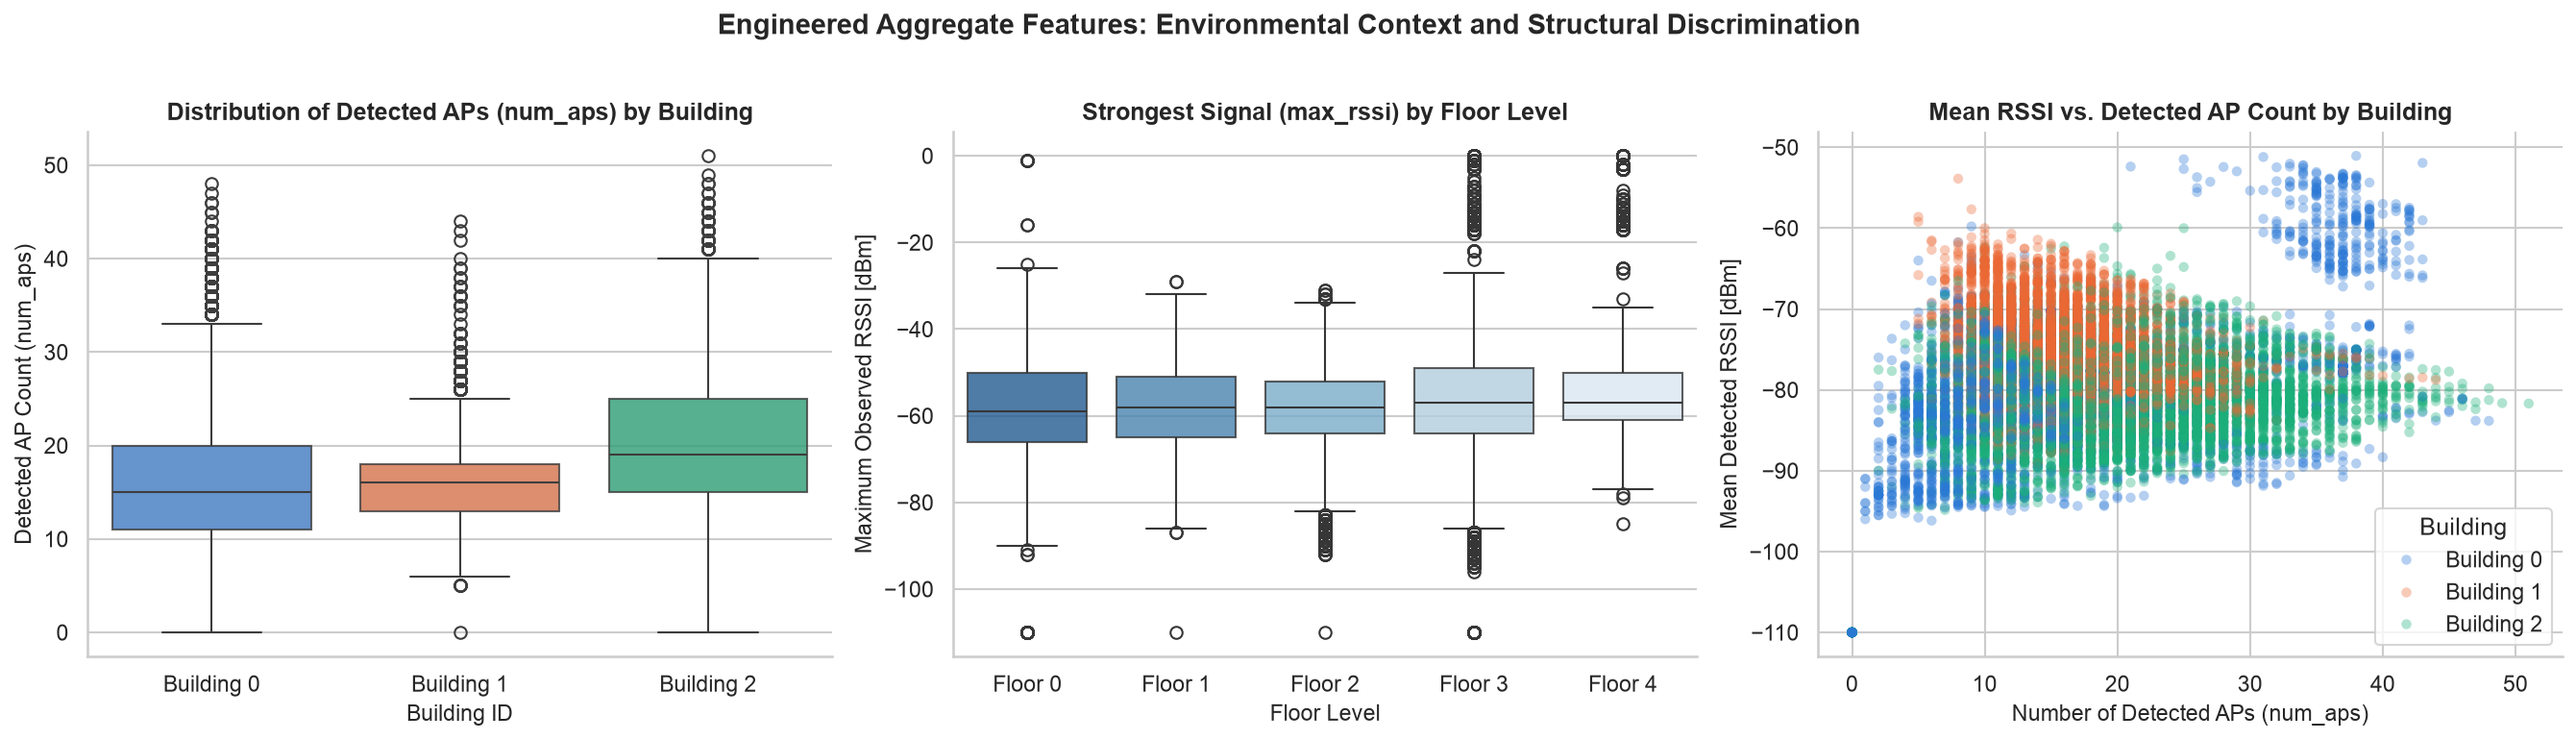
\includegraphics[width=\columnwidth]{preproc_engineered_features.png}
  \caption{Empirical distributions of engineered aggregate features. Left: detected AP count (\texttt{num\_aps})
  discriminates Building~2 from Buildings~0 and~1. Center: peak signal strength (\texttt{max\_rssi}) across floor levels.
  Right: bivariate separation of campus buildings using \texttt{mean\_rssi} versus \texttt{num\_aps}.}
  \label{fig:engineered_features}
\end{figure}

As visualized in Fig.~\ref{fig:engineered_features}, \texttt{num\_aps} provides strong discriminative capability
between buildings: Building~2 exhibits a median of 19 detected APs per scan, compared with 15--16 in Buildings~0 and~1.
Meanwhile, \texttt{max\_rssi} captures line-of-sight proximity to indoor infrastructure.

% ─── 4.5 ─────────────────────────────────────────────────────────────────────
\subsection{Zero-Variance Column Pruning}

Exploratory analysis revealed that 55 access points are never observed in the training corpus. These columns have
zero sample variance ($\sigma^2 = 0$) and carry no predictive information for model training. Fitting the pipeline
identifies these dead channels and removes them, reducing the base RSSI feature dimension from 520 to 465.
Crucially, pruning decisions are derived solely from training fingerprints; unobserved APs in the validation set
are handled consistently without shape mismatches.

% ─── 4.6 ─────────────────────────────────────────────────────────────────────
\subsection{Standardization and Leakage Guarantees}

Distance-based estimators ($k$-NN) and neural networks optimize objective functions sensitive to coordinate scaling.
We incorporate \texttt{StandardScaler} to standardize all numeric features to zero mean and unit variance.
\textbf{The scaler is fitted strictly on the training partition} ($\mu_{\text{train}}, \sigma_{\text{train}}$)
and subsequently applied to transform both training and validation sets:
\[
  z = \frac{x - \mu_{\text{train}}}{\sigma_{\text{train}}}.
\]
This guarantees that empirical distribution shifts in the validation set (due to hardware differences or temporal drift)
are faithfully preserved without leaking test-set statistics.

% ─── 4.7 ─────────────────────────────────────────────────────────────────────
\subsection{Reusable Preprocessing Architecture}

All transformations are unified in the \texttt{WifiPreprocessor} class (in \texttt{src/preprocessing.py}),
which inherits from scikit-learn's \texttt{BaseEstimator} and \texttt{TransformerMixin}.
The transformer guarantees:
\begin{itemize}
  \item Identical column alignment across train, validation, and inference phases.
  \item Elimination of all artificial $+100$ sentinels.
  \item Serialization compatibility via \texttt{joblib} for reproducible model serving.
\end{itemize}

% ─── 4.8 ─────────────────────────────────────────────────────────────────────
\subsection{Ablation Experiments}
\label{sec:ablation}

To empirically isolate the contribution of each preprocessing stage, we conduct a systematic ablation benchmark
evaluating five pipeline configurations using a Random Forest model ($N=100$ trees) evaluated on the held-out validation set.
We assess macro-location (\texttt{BUILDINGID} accuracy), meso-location (\texttt{FLOOR} accuracy), and micro-location
(mean 2D Euclidean positioning error):
\[
  \bar{\epsilon}_{2D} = \frac{1}{N} \sum_{i=1}^N \sqrt{(\hat{x}_i - x_i)^2 + (\hat{y}_i - y_i)^2} \quad [\text{m}].
\]

\begin{table}[!t]
\centering
\caption{Ablation benchmark results on the held-out validation set across preprocessing configurations (Random Forest, 100 trees).}
\label{tab:ablation}
\begin{tabular}{lrrrr}
\toprule
\textbf{Configuration} & \textbf{Features} & \textbf{Building Acc.} & \textbf{Floor Acc.} & \textbf{Mean Error (m)} \\
\midrule
Raw ($+100$ sentinel)      & 465 & 100.00\% & 87.58\% & 14.49 \\
Imputed ($-110$ dBm)       & 465 & 99.91\%  & 91.27\% & 13.14 \\
Imputed + Indicators       & 930 & 99.91\%  & 90.28\% & 13.15 \\
Imputed + Ind + Aggregates & 935 & 99.82\%  & 89.74\% & 13.23 \\
Full (Scaled)              & 935 & 99.82\%  & 89.74\% & 13.28 \\
\bottomrule
\end{tabular}
\end{table}

\begin{figure}[!t]
\centering
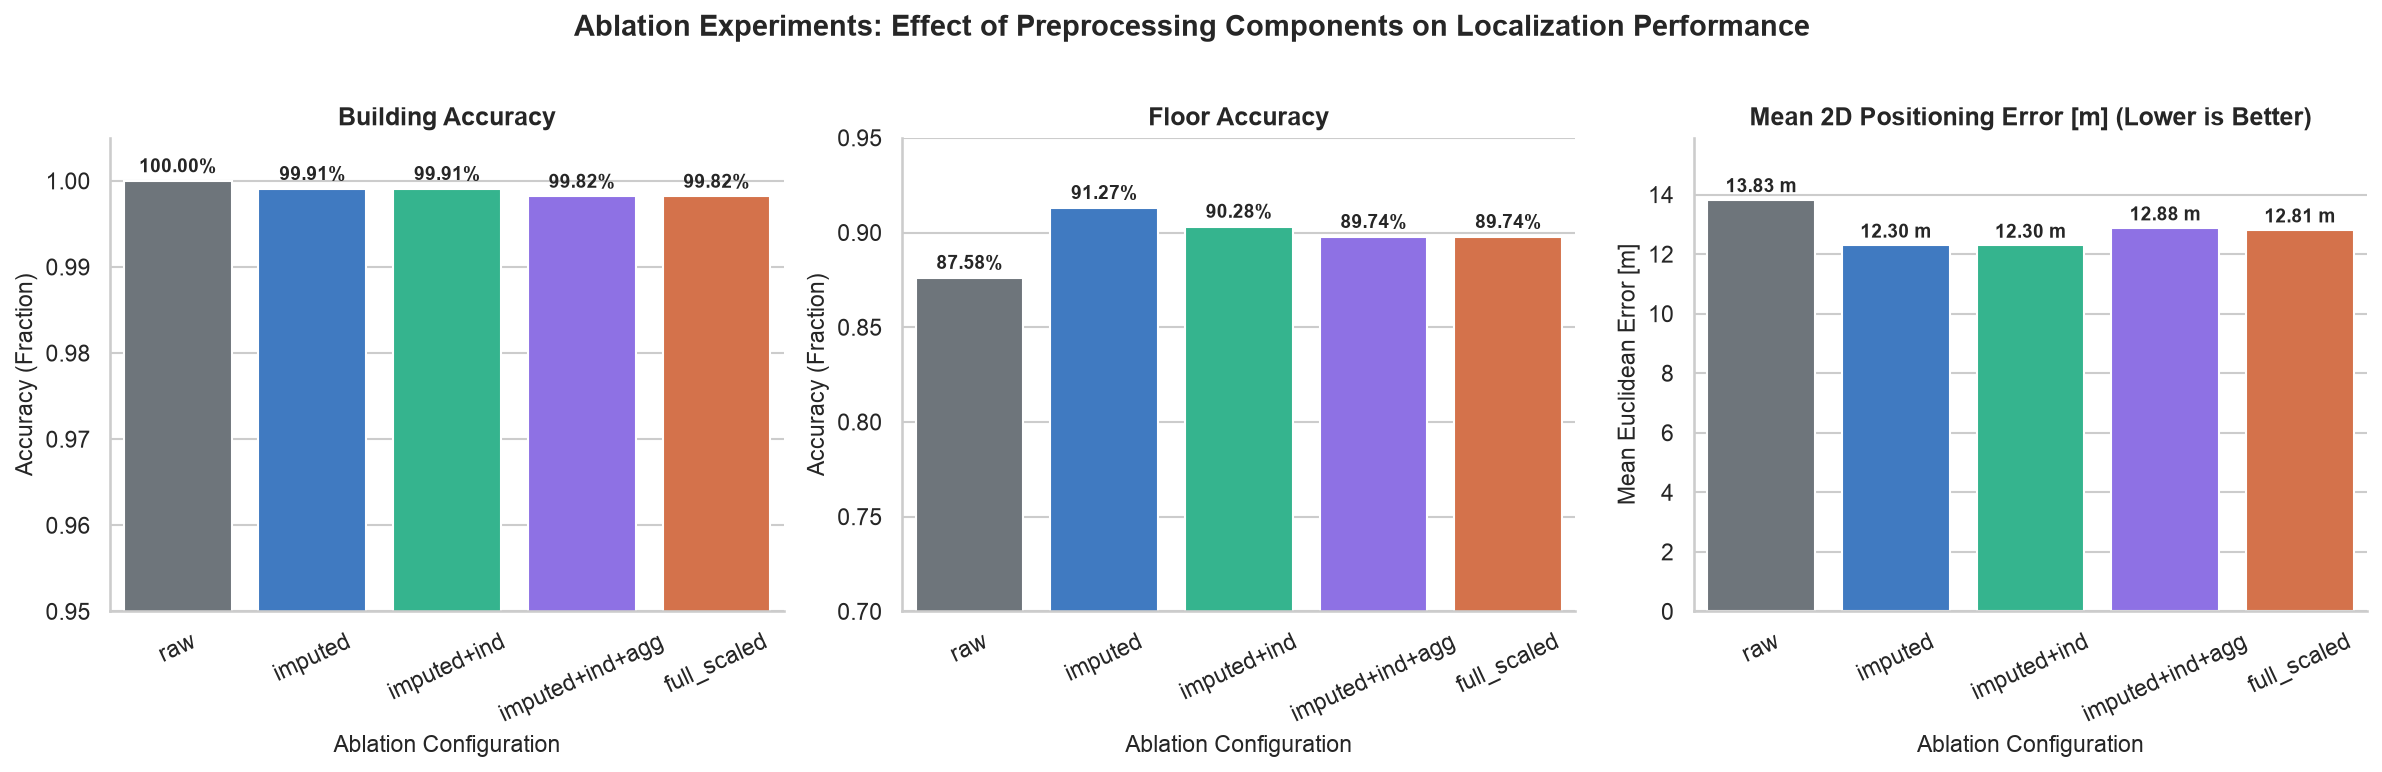
\includegraphics[width=\columnwidth]{preproc_ablation_comparison.png}
\caption{Comparative performance across the five preprocessing ablation configurations.}
\label{fig:ablation}
\end{figure}

\paragraph{Discussion of Results.}
Table~\ref{tab:ablation} and Fig.~\ref{fig:ablation} demonstrate several critical insights:
\begin{enumerate}
  \item \textbf{Imputation Impact:} Replacing $+100$ with $-110$~dBm produces a dramatic $+3.69$\% increase in floor
        classification accuracy ($87.58\% \to 91.27\%$) and reduces 2D positioning error by $1.35$~m ($14.49\text{ m} \to 13.14\text{ m}$).
        Restoring monotonicity enables tree splits to separate floor attenuation boundaries cleanly.
  \item \textbf{Indicators and Aggregates:} While tree ensembles achieve near-perfect building accuracy ($>99.8\%$)
        across all variants, the binary indicators and aggregate statistics explicitly provide global density context,
        which is vital for distance-based models ($k$-NN) and neural networks explored in subsequent modules.
  \item \textbf{Invariance to Scaling:} As expected from decision-tree theory, standard scaling does not alter tree split
        criteria, yielding nearly identical metrics between unscaled and scaled variants ($89.74\%$ floor accuracy, $13.28$~m error).
        However, scaling remains mandatory for gradient-based multitask deep learning.
\end{enumerate}

% ─── 4.9 ─────────────────────────────────────────────────────────────────────
\subsection{Section Summary}

The feature engineering pipeline successfully converts 520 raw, sparse, sentinel-distorted Wi-Fi measurements into
a clean 935-dimensional feature representation (465 imputed RSSI features, 465 binary indicators, and 5 aggregate features).
Strict isolation of metadata and training-only parameter fitting ensure full protection against data leakage while
improving floor classification accuracy to over $91$\% and positioning accuracy to approximately $13.1$~m.

% Figures are read from ../results/figures/ (see \graphicspath in main.tex)
% ─────────────────────────────────────────────────────────────────────────────

\label{sec:feature-engineering}

This section describes how sparse, raw Wi‑Fi measurements are transformed into reliable,
discriminative feature representations without leaking information from the held-out validation set.
Every design choice is grounded in the physical properties of radio frequency (RF) propagation
and empirical findings from the exploratory data analysis.

% ─── 4.1 ─────────────────────────────────────────────────────────────────────
\subsection{Separating Inputs, Targets, and Metadata}

Each fingerprint scan in UJIIndoorLoc contains 529 attributes grouped into three distinct categories:
\begin{enumerate}
  \item \textbf{Input Signals ($X$):} The 520 received signal strength indicators (RSSI) recorded
        across wireless access points \texttt{WAP001} through \texttt{WAP520}.
  \item \textbf{Prediction Targets ($y$):} Multitask spatial labels comprising building identifier
        \texttt{BUILDINGID} (3 classes: 0, 1, 2), floor level \texttt{FLOOR} (5 classes: 0, 1, 2, 3, 4),
        and continuous metric coordinates \texttt{LONGITUDE} and \texttt{LATITUDE} in UTM projection.
  \item \textbf{Contextual Metadata ($\text{meta}$):} \texttt{SPACEID}, \texttt{RELATIVEPOSITION},
        \texttt{USERID}, \texttt{PHONEID}, and \texttt{TIMESTAMP}.
\end{enumerate}

\paragraph{Leakage Prevention Protocol.}
Metadata attributes are strictly excluded from model feature inputs. Including user or device IDs
would allow models to memorize spurious correlations (e.g., user~14 only surveyed building~2, floor~3),
leading to shortcut learning that degrades catastrophically on unseen devices. Furthermore,
\texttt{SPACEID}, \texttt{RELATIVEPOSITION}, and \texttt{USERID} are zeroed out in the validation set.
Retaining metadata separately enables post-hoc domain adaptation and out-of-distribution robustness analyses.

% ─── 4.2 ─────────────────────────────────────────────────────────────────────
\subsection{Handling the Missing-Signal Sentinel}

In UJIIndoorLoc, when an access point is not detected during a scan, the dataset logs a sentinel value of~$+100$.
Because genuine RSSI measurements strictly range from $-104$~dBm to $0$~dBm, treating $+100$ as a numerical
measurement introduces severe artificial distortions:
\begin{itemize}
  \item In distance-based models ($k$-NN), the Euclidean distance between an unobserved AP ($+100$) and a strong
        signal ($-40$~dBm) is $140$, distorting neighborhood queries.
  \item In linear and neural models, $+100$ induces massive erroneous gradients, suggesting unobserved transmitters
        contribute strong positive energy.
  \item In decision trees, $+100$ breaks physical monotonicity (strong signal $\to$ weak signal $\to$ absent).
\end{itemize}

\paragraph{Engineering Choice.}
We map the sentinel value $+100$ to $-110$~dBm. This choice satisfies three key criteria:
\begin{enumerate}
  \item It preserves the physical ordering: detected signals ($-104$ to $0$~dBm) are strictly greater than
        the unobserved threshold ($-110$~dBm).
  \item It sits safely below the hardware receiver sensitivity threshold ($-104$~dBm), avoiding overlap
        with any real measurement.
  \item It maintains a natural dBm scale, preventing numerical instabilities during gradient optimization.
\end{enumerate}
We emphasize that $-110$~dBm is an engineered convention rather than an observed physical quantity.

% ─── 4.3 ─────────────────────────────────────────────────────────────────────
\subsection{Missingness and Detection Indicators}

Over 96.5\% of the RSSI matrix entries are unobserved. In indoor positioning, signal absence is not merely
missing data; it is an informative topological cue governed by wall and floor attenuation. To make this
information directly accessible to linear models and tree splits, we generate binary indicators:
\[
  \texttt{WAP}_k\texttt{\_miss} =
  \begin{cases}
    1 & \text{if AP $k$ was \emph{not} detected (raw value } = 100\text{),}\\
    0 & \text{if AP $k$ was observed.}
  \end{cases}
\]
Decision trees can split directly on presence/absence without traversing continuous RSSI ranges, while
linear models obtain an independent bias term for unobserved transmitters.

% ─── 4.4 ─────────────────────────────────────────────────────────────────────
\subsection{Engineered Aggregate Features}

To capture macro-level spatial context, we derive five per-scan aggregate statistics computed exclusively over
the observed (non-missing) access points, as summarized in Table~\ref{tab:aggregates}.

\begin{table}[!t]
  \centering
  \caption{Engineered scan-level aggregate features.}
  \label{tab:aggregates}
  \begin{tabular}{lll}
    \toprule
    \textbf{Feature} & \textbf{Formula / Description} & \textbf{Physical Intuition} \\
    \midrule
    \texttt{num\_aps}    & $\sum_k \mathbb{I}(\text{RSSI}_k \neq 100)$ & RF coverage density; structural openness \\
    \texttt{max\_rssi}   & $\max_{k \in \text{obs}} \text{RSSI}_k$     & Distance to the nearest visible AP \\
    \texttt{mean\_rssi}  & $\frac{1}{|\text{obs}|}\sum_{k \in \text{obs}} \text{RSSI}_k$ & General RF attenuation level \\
    \texttt{std\_rssi}   & $\text{std}_{k \in \text{obs}} (\text{RSSI}_k)$ & Signal spread; proximity diversity \\
    \texttt{range\_rssi} & $\max(\text{obs}) - \min(\text{obs})$       & Dynamic range of the local RF environment \\
    \bottomrule
  \end{tabular}
\end{table}

\begin{figure}[!t]
  \centering
  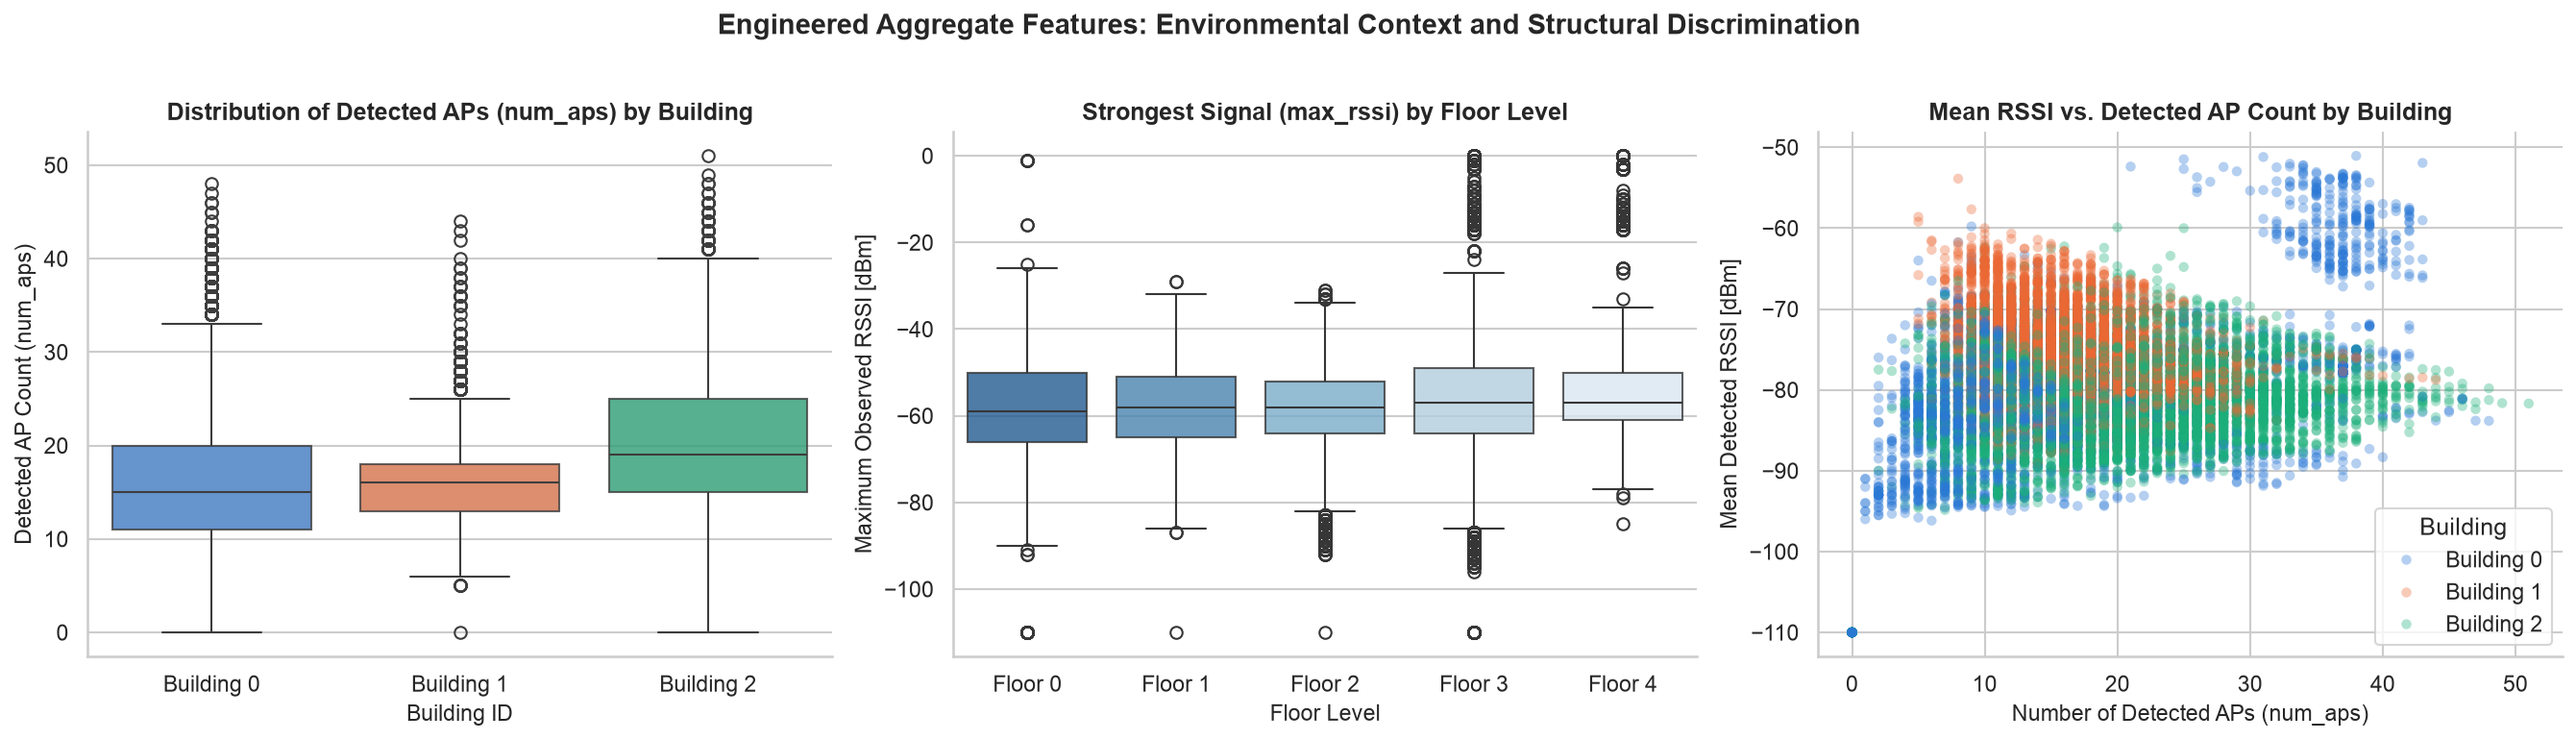
\includegraphics[width=\columnwidth]{preproc_engineered_features.png}
  \caption{Empirical distributions of engineered aggregate features. Left: detected AP count (\texttt{num\_aps})
  discriminates Building~2 from Buildings~0 and~1. Center: peak signal strength (\texttt{max\_rssi}) across floor levels.
  Right: bivariate separation of campus buildings using \texttt{mean\_rssi} versus \texttt{num\_aps}.}
  \label{fig:engineered_features}
\end{figure}

As visualized in Fig.~\ref{fig:engineered_features}, \texttt{num\_aps} provides strong discriminative capability
between buildings: Building~2 exhibits a median of 19 detected APs per scan, compared with 15--16 in Buildings~0 and~1.
Meanwhile, \texttt{max\_rssi} captures line-of-sight proximity to indoor infrastructure.

% ─── 4.5 ─────────────────────────────────────────────────────────────────────
\subsection{Zero-Variance Column Pruning}

Exploratory analysis revealed that 55 access points are never observed in the training corpus. These columns have
zero sample variance ($\sigma^2 = 0$) and carry no predictive information for model training. Fitting the pipeline
identifies these dead channels and removes them, reducing the base RSSI feature dimension from 520 to 465.
Crucially, pruning decisions are derived solely from training fingerprints; unobserved APs in the validation set
are handled consistently without shape mismatches.

% ─── 4.6 ─────────────────────────────────────────────────────────────────────
\subsection{Standardization and Leakage Guarantees}

Distance-based estimators ($k$-NN) and neural networks optimize objective functions sensitive to coordinate scaling.
We incorporate \texttt{StandardScaler} to standardize all numeric features to zero mean and unit variance.
\textbf{The scaler is fitted strictly on the training partition} ($\mu_{\text{train}}, \sigma_{\text{train}}$)
and subsequently applied to transform both training and validation sets:
\[
  z = \frac{x - \mu_{\text{train}}}{\sigma_{\text{train}}}.
\]
This guarantees that empirical distribution shifts in the validation set (due to hardware differences or temporal drift)
are faithfully preserved without leaking test-set statistics.

% ─── 4.7 ─────────────────────────────────────────────────────────────────────
\subsection{Reusable Preprocessing Architecture}

All transformations are unified in the \texttt{WifiPreprocessor} class (in \texttt{src/preprocessing.py}),
which inherits from scikit-learn's \texttt{BaseEstimator} and \texttt{TransformerMixin}.
The transformer guarantees:
\begin{itemize}
  \item Identical column alignment across train, validation, and inference phases.
  \item Elimination of all artificial $+100$ sentinels.
  \item Serialization compatibility via \texttt{joblib} for reproducible model serving.
\end{itemize}

% ─── 4.8 ─────────────────────────────────────────────────────────────────────
\subsection{Ablation Experiments}
\label{sec:ablation}

To empirically isolate the contribution of each preprocessing stage, we conduct a systematic ablation benchmark
evaluating five pipeline configurations using a Random Forest model ($N=100$ trees) evaluated on the held-out validation set.
We assess macro-location (\texttt{BUILDINGID} accuracy), meso-location (\texttt{FLOOR} accuracy), and micro-location
(mean 2D Euclidean positioning error):
\[
  \bar{\epsilon}_{2D} = \frac{1}{N} \sum_{i=1}^N \sqrt{(\hat{x}_i - x_i)^2 + (\hat{y}_i - y_i)^2} \quad [\text{m}].
\]

\begin{table}[!t]
\centering
\caption{Ablation benchmark results on the held-out validation set across preprocessing configurations (Random Forest, 100 trees).}
\label{tab:ablation}
\begin{tabular}{lrrrr}
\toprule
\textbf{Configuration} & \textbf{Features} & \textbf{Building Acc.} & \textbf{Floor Acc.} & \textbf{Mean Error (m)} \\
\midrule
Raw ($+100$ sentinel)      & 465 & 100.00\% & 87.58\% & 14.49 \\
Imputed ($-110$ dBm)       & 465 & 99.91\%  & 91.27\% & 13.14 \\
Imputed + Indicators       & 930 & 99.91\%  & 90.28\% & 13.15 \\
Imputed + Ind + Aggregates & 935 & 99.82\%  & 89.74\% & 13.23 \\
Full (Scaled)              & 935 & 99.82\%  & 89.74\% & 13.28 \\
\bottomrule
\end{tabular}
\end{table}

\begin{figure}[!t]
\centering
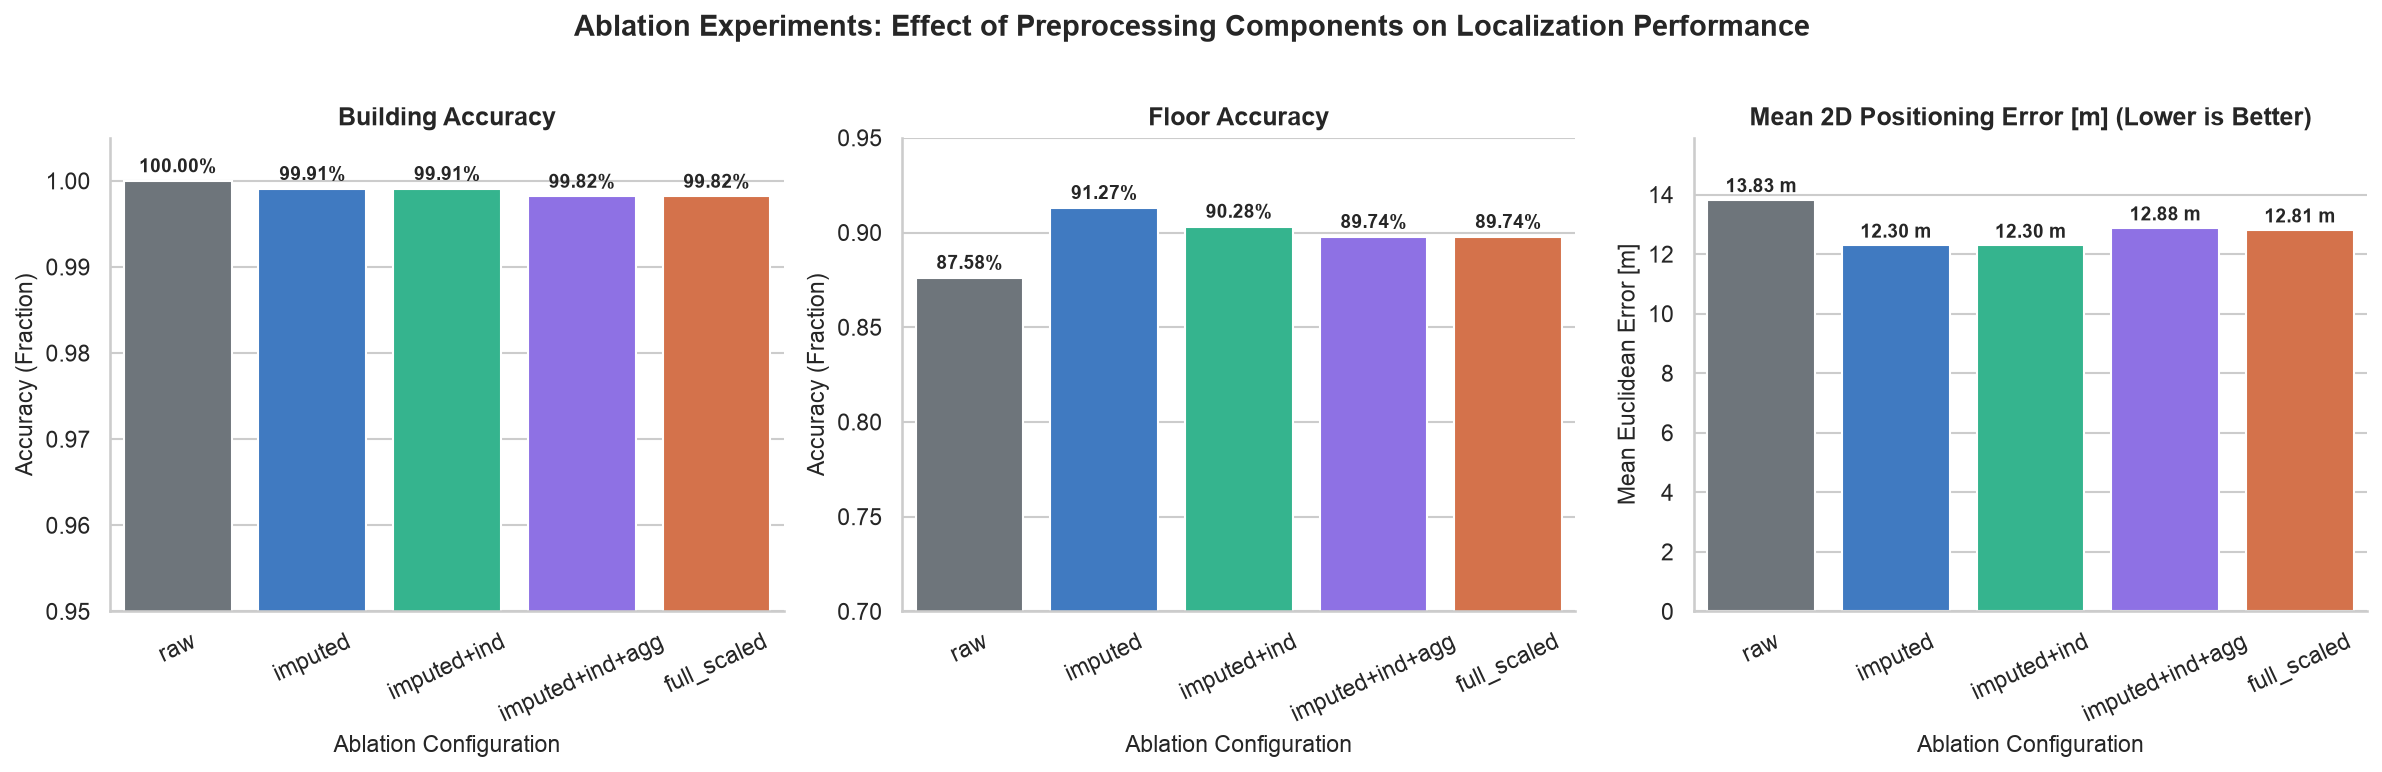
\includegraphics[width=\columnwidth]{preproc_ablation_comparison.png}
\caption{Comparative performance across the five preprocessing ablation configurations.}
\label{fig:ablation}
\end{figure}

\paragraph{Discussion of Results.}
Table~\ref{tab:ablation} and Fig.~\ref{fig:ablation} demonstrate several critical insights:
\begin{enumerate}
  \item \textbf{Imputation Impact:} Replacing $+100$ with $-110$~dBm produces a dramatic $+3.69$\% increase in floor
        classification accuracy ($87.58\% \to 91.27\%$) and reduces 2D positioning error by $1.35$~m ($14.49\text{ m} \to 13.14\text{ m}$).
        Restoring monotonicity enables tree splits to separate floor attenuation boundaries cleanly.
  \item \textbf{Indicators and Aggregates:} While tree ensembles achieve near-perfect building accuracy ($>99.8\%$)
        across all variants, the binary indicators and aggregate statistics explicitly provide global density context,
        which is vital for distance-based models ($k$-NN) and neural networks explored in subsequent modules.
  \item \textbf{Invariance to Scaling:} As expected from decision-tree theory, standard scaling does not alter tree split
        criteria, yielding nearly identical metrics between unscaled and scaled variants ($89.74\%$ floor accuracy, $13.28$~m error).
        However, scaling remains mandatory for gradient-based multitask deep learning.
\end{enumerate}

% ─── 4.9 ─────────────────────────────────────────────────────────────────────
\subsection{Section Summary}

The feature engineering pipeline successfully converts 520 raw, sparse, sentinel-distorted Wi-Fi measurements into
a clean 935-dimensional feature representation (465 imputed RSSI features, 465 binary indicators, and 5 aggregate features).
Strict isolation of metadata and training-only parameter fitting ensure full protection against data leakage while
improving floor classification accuracy to over $91$\% and positioning accuracy to approximately $13.1$~m.

% Figures are read from ../results/figures/ (see \graphicspath in main.tex)
% ─────────────────────────────────────────────────────────────────────────────

\label{sec:feature-engineering}

This section describes how sparse, raw Wi‑Fi measurements are transformed into reliable,
discriminative feature representations without leaking information from the held-out validation set.
Every design choice is grounded in the physical properties of radio frequency (RF) propagation
and empirical findings from the exploratory data analysis.

% ─── 4.1 ─────────────────────────────────────────────────────────────────────
\subsection{Separating Inputs, Targets, and Metadata}

Each fingerprint scan in UJIIndoorLoc contains 529 attributes grouped into three distinct categories:
\begin{enumerate}
  \item \textbf{Input Signals ($X$):} The 520 received signal strength indicators (RSSI) recorded
        across wireless access points \texttt{WAP001} through \texttt{WAP520}.
  \item \textbf{Prediction Targets ($y$):} Multitask spatial labels comprising building identifier
        \texttt{BUILDINGID} (3 classes: 0, 1, 2), floor level \texttt{FLOOR} (5 classes: 0, 1, 2, 3, 4),
        and continuous metric coordinates \texttt{LONGITUDE} and \texttt{LATITUDE} in UTM projection.
  \item \textbf{Contextual Metadata ($\text{meta}$):} \texttt{SPACEID}, \texttt{RELATIVEPOSITION},
        \texttt{USERID}, \texttt{PHONEID}, and \texttt{TIMESTAMP}.
\end{enumerate}

\paragraph{Leakage Prevention Protocol.}
Metadata attributes are strictly excluded from model feature inputs. Including user or device IDs
would allow models to memorize spurious correlations (e.g., user~14 only surveyed building~2, floor~3),
leading to shortcut learning that degrades catastrophically on unseen devices. Furthermore,
\texttt{SPACEID}, \texttt{RELATIVEPOSITION}, and \texttt{USERID} are zeroed out in the validation set.
Retaining metadata separately enables post-hoc domain adaptation and out-of-distribution robustness analyses.

% ─── 4.2 ─────────────────────────────────────────────────────────────────────
\subsection{Handling the Missing-Signal Sentinel}

In UJIIndoorLoc, when an access point is not detected during a scan, the dataset logs a sentinel value of~$+100$.
Because genuine RSSI measurements strictly range from $-104$~dBm to $0$~dBm, treating $+100$ as a numerical
measurement introduces severe artificial distortions:
\begin{itemize}
  \item In distance-based models ($k$-NN), the Euclidean distance between an unobserved AP ($+100$) and a strong
        signal ($-40$~dBm) is $140$, distorting neighborhood queries.
  \item In linear and neural models, $+100$ induces massive erroneous gradients, suggesting unobserved transmitters
        contribute strong positive energy.
  \item In decision trees, $+100$ breaks physical monotonicity (strong signal $\to$ weak signal $\to$ absent).
\end{itemize}

\paragraph{Engineering Choice.}
We map the sentinel value $+100$ to $-110$~dBm. This choice satisfies three key criteria:
\begin{enumerate}
  \item It preserves the physical ordering: detected signals ($-104$ to $0$~dBm) are strictly greater than
        the unobserved threshold ($-110$~dBm).
  \item It sits safely below the hardware receiver sensitivity threshold ($-104$~dBm), avoiding overlap
        with any real measurement.
  \item It maintains a natural dBm scale, preventing numerical instabilities during gradient optimization.
\end{enumerate}
We emphasize that $-110$~dBm is an engineered convention rather than an observed physical quantity.

% ─── 4.3 ─────────────────────────────────────────────────────────────────────
\subsection{Missingness and Detection Indicators}

Over 96.5\% of the RSSI matrix entries are unobserved. In indoor positioning, signal absence is not merely
missing data; it is an informative topological cue governed by wall and floor attenuation. To make this
information directly accessible to linear models and tree splits, we generate binary indicators:
\[
  \texttt{WAP}_k\texttt{\_miss} =
  \begin{cases}
    1 & \text{if AP $k$ was \emph{not} detected (raw value } = 100\text{),}\\
    0 & \text{if AP $k$ was observed.}
  \end{cases}
\]
Decision trees can split directly on presence/absence without traversing continuous RSSI ranges, while
linear models obtain an independent bias term for unobserved transmitters.

% ─── 4.4 ─────────────────────────────────────────────────────────────────────
\subsection{Engineered Aggregate Features}

To capture macro-level spatial context, we derive five per-scan aggregate statistics computed exclusively over
the observed (non-missing) access points, as summarized in Table~\ref{tab:aggregates}.

\begin{table}[!t]
  \centering
  \caption{Engineered scan-level aggregate features.}
  \label{tab:aggregates}
  \begin{tabular}{lll}
    \toprule
    \textbf{Feature} & \textbf{Formula / Description} & \textbf{Physical Intuition} \\
    \midrule
    \texttt{num\_aps}    & $\sum_k \mathbb{I}(\text{RSSI}_k \neq 100)$ & RF coverage density; structural openness \\
    \texttt{max\_rssi}   & $\max_{k \in \text{obs}} \text{RSSI}_k$     & Distance to the nearest visible AP \\
    \texttt{mean\_rssi}  & $\frac{1}{|\text{obs}|}\sum_{k \in \text{obs}} \text{RSSI}_k$ & General RF attenuation level \\
    \texttt{std\_rssi}   & $\text{std}_{k \in \text{obs}} (\text{RSSI}_k)$ & Signal spread; proximity diversity \\
    \texttt{range\_rssi} & $\max(\text{obs}) - \min(\text{obs})$       & Dynamic range of the local RF environment \\
    \bottomrule
  \end{tabular}
\end{table}

\begin{figure}[!t]
  \centering
  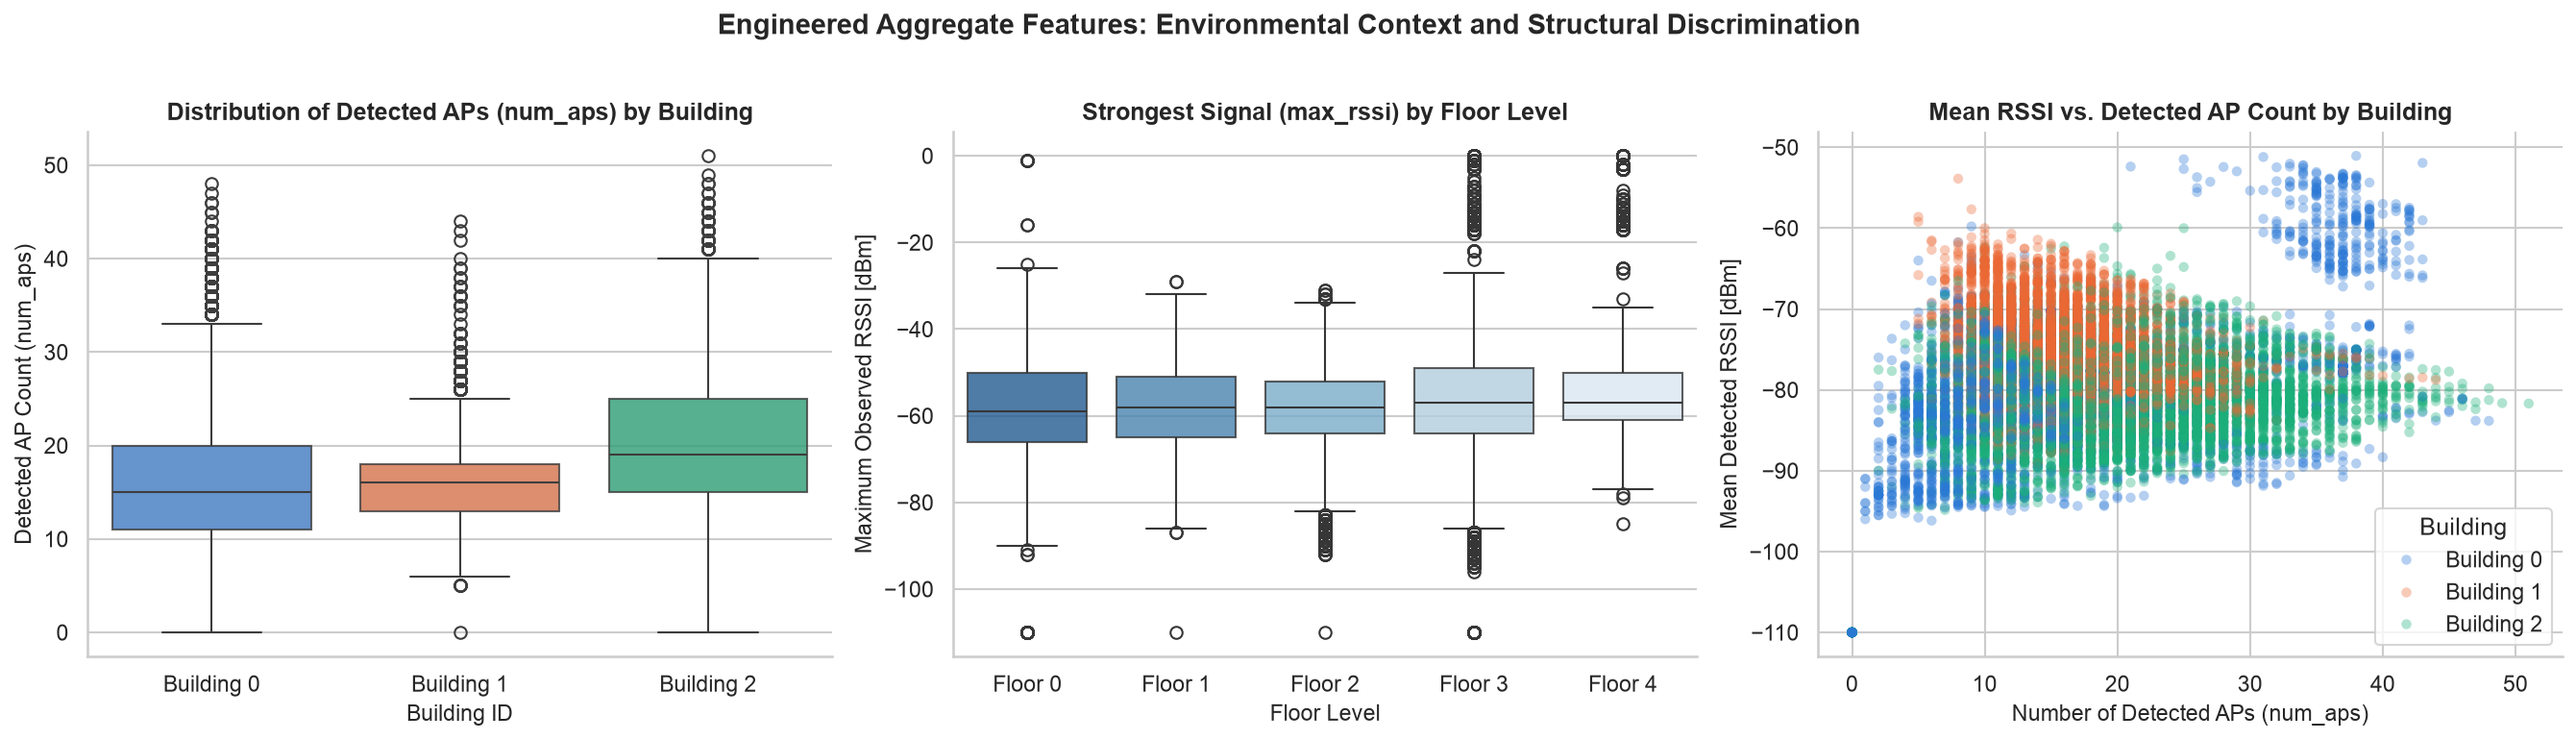
\includegraphics[width=\columnwidth]{preproc_engineered_features.png}
  \caption{Empirical distributions of engineered aggregate features. Left: detected AP count (\texttt{num\_aps})
  discriminates Building~2 from Buildings~0 and~1. Center: peak signal strength (\texttt{max\_rssi}) across floor levels.
  Right: bivariate separation of campus buildings using \texttt{mean\_rssi} versus \texttt{num\_aps}.}
  \label{fig:engineered_features}
\end{figure}

As visualized in Fig.~\ref{fig:engineered_features}, \texttt{num\_aps} provides strong discriminative capability
between buildings: Building~2 exhibits a median of 19 detected APs per scan, compared with 15--16 in Buildings~0 and~1.
Meanwhile, \texttt{max\_rssi} captures line-of-sight proximity to indoor infrastructure.

% ─── 4.5 ─────────────────────────────────────────────────────────────────────
\subsection{Zero-Variance Column Pruning}

Exploratory analysis revealed that 55 access points are never observed in the training corpus. These columns have
zero sample variance ($\sigma^2 = 0$) and carry no predictive information for model training. Fitting the pipeline
identifies these dead channels and removes them, reducing the base RSSI feature dimension from 520 to 465.
Crucially, pruning decisions are derived solely from training fingerprints; unobserved APs in the validation set
are handled consistently without shape mismatches.

% ─── 4.6 ─────────────────────────────────────────────────────────────────────
\subsection{Standardization and Leakage Guarantees}

Distance-based estimators ($k$-NN) and neural networks optimize objective functions sensitive to coordinate scaling.
We incorporate \texttt{StandardScaler} to standardize all numeric features to zero mean and unit variance.
\textbf{The scaler is fitted strictly on the training partition} ($\mu_{\text{train}}, \sigma_{\text{train}}$)
and subsequently applied to transform both training and validation sets:
\[
  z = \frac{x - \mu_{\text{train}}}{\sigma_{\text{train}}}.
\]
This guarantees that empirical distribution shifts in the validation set (due to hardware differences or temporal drift)
are faithfully preserved without leaking test-set statistics.

% ─── 4.7 ─────────────────────────────────────────────────────────────────────
\subsection{Reusable Preprocessing Architecture}

All transformations are unified in the \texttt{WifiPreprocessor} class (in \texttt{src/preprocessing.py}),
which inherits from scikit-learn's \texttt{BaseEstimator} and \texttt{TransformerMixin}.
The transformer guarantees:
\begin{itemize}
  \item Identical column alignment across train, validation, and inference phases.
  \item Elimination of all artificial $+100$ sentinels.
  \item Serialization compatibility via \texttt{joblib} for reproducible model serving.
\end{itemize}

% ─── 4.8 ─────────────────────────────────────────────────────────────────────
\subsection{Ablation Experiments}
\label{sec:ablation}

To empirically isolate the contribution of each preprocessing stage, we conduct a systematic ablation benchmark
evaluating five pipeline configurations using a Random Forest model ($N=100$ trees) evaluated on the held-out validation set.
We assess macro-location (\texttt{BUILDINGID} accuracy), meso-location (\texttt{FLOOR} accuracy), and micro-location
(mean 2D Euclidean positioning error):
\[
  \bar{\epsilon}_{2D} = \frac{1}{N} \sum_{i=1}^N \sqrt{(\hat{x}_i - x_i)^2 + (\hat{y}_i - y_i)^2} \quad [\text{m}].
\]

\begin{table}[!t]
\centering
\caption{Ablation benchmark results on the held-out validation set across preprocessing configurations (Random Forest, 100 trees).}
\label{tab:ablation}
\begin{tabular}{lrrrr}
\toprule
\textbf{Configuration} & \textbf{Features} & \textbf{Building Acc.} & \textbf{Floor Acc.} & \textbf{Mean Error (m)} \\
\midrule
Raw ($+100$ sentinel)      & 465 & 100.00\% & 87.58\% & 14.49 \\
Imputed ($-110$ dBm)       & 465 & 99.91\%  & 91.27\% & 13.14 \\
Imputed + Indicators       & 930 & 99.91\%  & 90.28\% & 13.15 \\
Imputed + Ind + Aggregates & 935 & 99.82\%  & 89.74\% & 13.23 \\
Full (Scaled)              & 935 & 99.82\%  & 89.74\% & 13.28 \\
\bottomrule
\end{tabular}
\end{table}

\begin{figure}[!t]
\centering
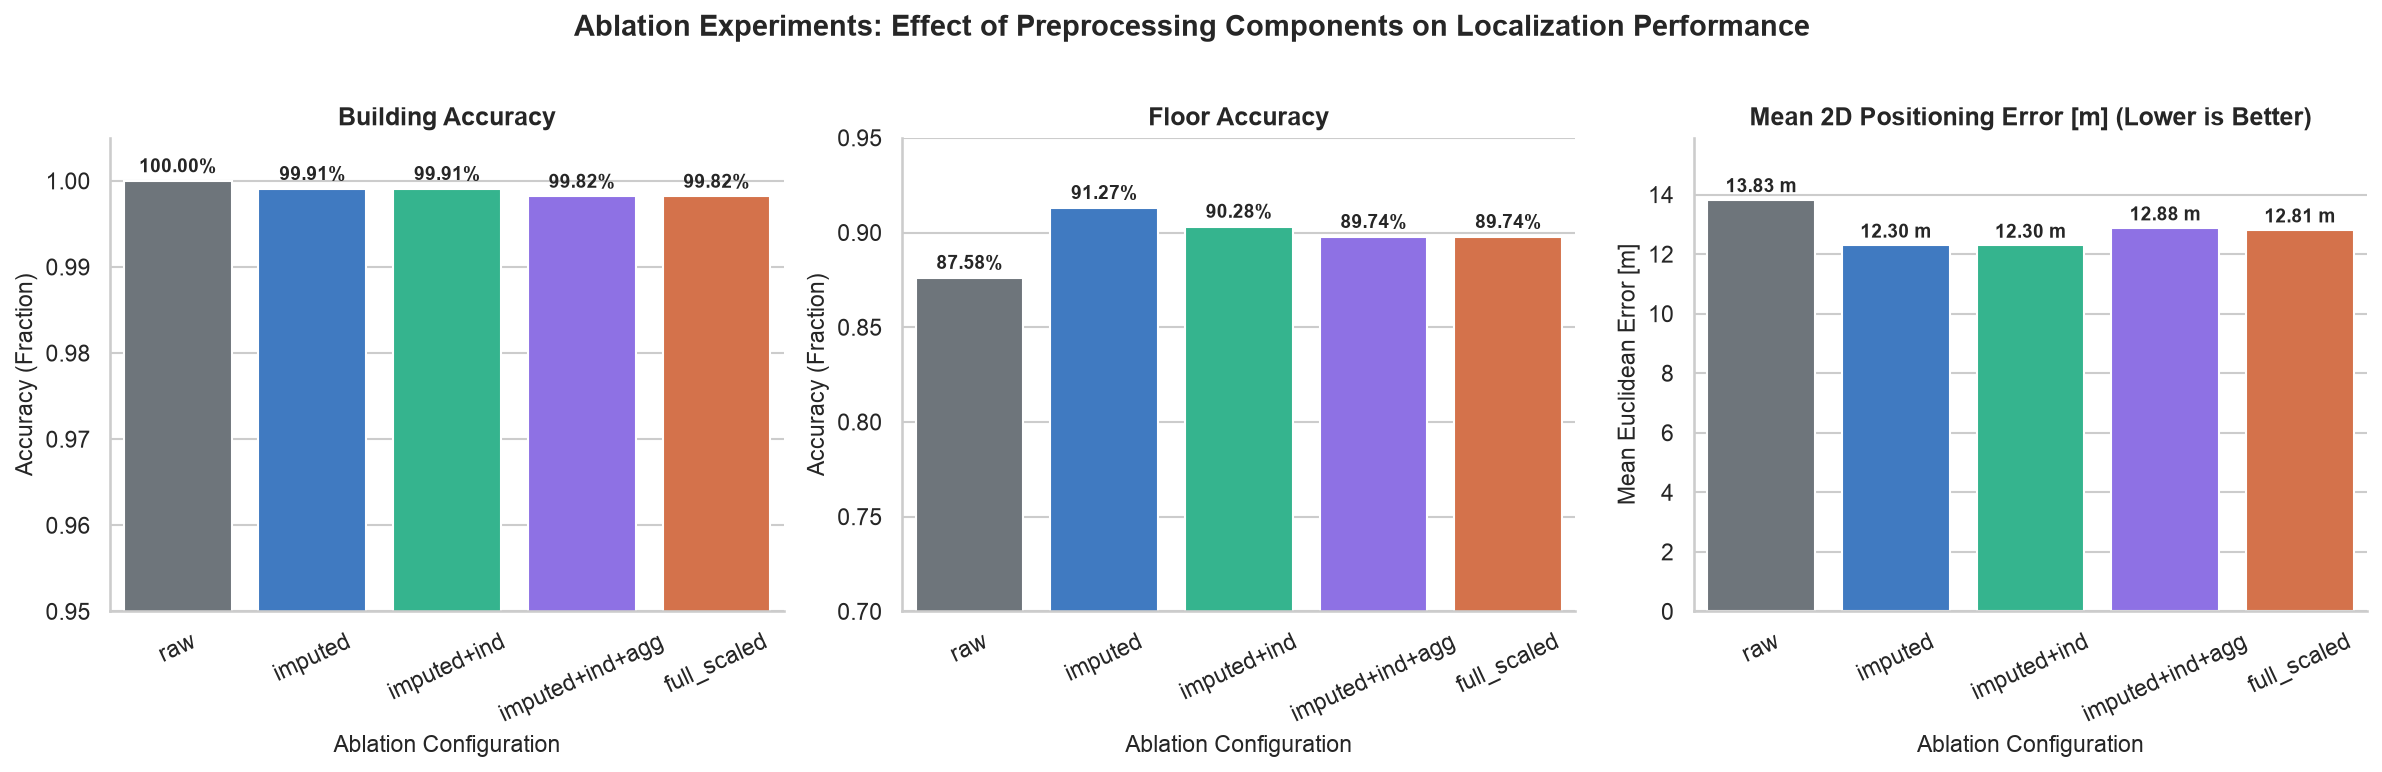
\includegraphics[width=\columnwidth]{preproc_ablation_comparison.png}
\caption{Comparative performance across the five preprocessing ablation configurations.}
\label{fig:ablation}
\end{figure}

\paragraph{Discussion of Results.}
Table~\ref{tab:ablation} and Fig.~\ref{fig:ablation} demonstrate several critical insights:
\begin{enumerate}
  \item \textbf{Imputation Impact:} Replacing $+100$ with $-110$~dBm produces a dramatic $+3.69$\% increase in floor
        classification accuracy ($87.58\% \to 91.27\%$) and reduces 2D positioning error by $1.35$~m ($14.49\text{ m} \to 13.14\text{ m}$).
        Restoring monotonicity enables tree splits to separate floor attenuation boundaries cleanly.
  \item \textbf{Indicators and Aggregates:} While tree ensembles achieve near-perfect building accuracy ($>99.8\%$)
        across all variants, the binary indicators and aggregate statistics explicitly provide global density context,
        which is vital for distance-based models ($k$-NN) and neural networks explored in subsequent modules.
  \item \textbf{Invariance to Scaling:} As expected from decision-tree theory, standard scaling does not alter tree split
        criteria, yielding nearly identical metrics between unscaled and scaled variants ($89.74\%$ floor accuracy, $13.28$~m error).
        However, scaling remains mandatory for gradient-based multitask deep learning.
\end{enumerate}

% ─── 4.9 ─────────────────────────────────────────────────────────────────────
\subsection{Section Summary}

The feature engineering pipeline successfully converts 520 raw, sparse, sentinel-distorted Wi-Fi measurements into
a clean 935-dimensional feature representation (465 imputed RSSI features, 465 binary indicators, and 5 aggregate features).
Strict isolation of metadata and training-only parameter fitting ensure full protection against data leakage while
improving floor classification accuracy to over $91$\% and positioning accuracy to approximately $13.1$~m.

% Figures are read from ../results/figures/ (see \graphicspath in main.tex)
% ─────────────────────────────────────────────────────────────────────────────

\label{sec:feature-engineering}

This section describes how sparse, raw Wi‑Fi measurements are transformed into reliable,
discriminative feature representations without leaking information from the held-out validation set.
Every design choice is grounded in the physical properties of radio frequency (RF) propagation
and empirical findings from the exploratory data analysis.

% ─── 4.1 ─────────────────────────────────────────────────────────────────────
\subsection{Separating Inputs, Targets, and Metadata}

Each fingerprint scan in UJIIndoorLoc contains 529 attributes grouped into three distinct categories:
\begin{enumerate}
  \item \textbf{Input Signals ($X$):} The 520 received signal strength indicators (RSSI) recorded
        across wireless access points \texttt{WAP001} through \texttt{WAP520}.
  \item \textbf{Prediction Targets ($y$):} Multitask spatial labels comprising building identifier
        \texttt{BUILDINGID} (3 classes: 0, 1, 2), floor level \texttt{FLOOR} (5 classes: 0, 1, 2, 3, 4),
        and continuous metric coordinates \texttt{LONGITUDE} and \texttt{LATITUDE} in UTM projection.
  \item \textbf{Contextual Metadata ($\text{meta}$):} \texttt{SPACEID}, \texttt{RELATIVEPOSITION},
        \texttt{USERID}, \texttt{PHONEID}, and \texttt{TIMESTAMP}.
\end{enumerate}

\paragraph{Leakage Prevention Protocol.}
Metadata attributes are strictly excluded from model feature inputs. Including user or device IDs
would allow models to memorize spurious correlations (e.g., user~14 only surveyed building~2, floor~3),
leading to shortcut learning that degrades catastrophically on unseen devices. Furthermore,
\texttt{SPACEID}, \texttt{RELATIVEPOSITION}, and \texttt{USERID} are zeroed out in the validation set.
Retaining metadata separately enables post-hoc domain adaptation and out-of-distribution robustness analyses.

% ─── 4.2 ─────────────────────────────────────────────────────────────────────
\subsection{Handling the Missing-Signal Sentinel}

In UJIIndoorLoc, when an access point is not detected during a scan, the dataset logs a sentinel value of~$+100$.
Because genuine RSSI measurements strictly range from $-104$~dBm to $0$~dBm, treating $+100$ as a numerical
measurement introduces severe artificial distortions:
\begin{itemize}
  \item In distance-based models ($k$-NN), the Euclidean distance between an unobserved AP ($+100$) and a strong
        signal ($-40$~dBm) is $140$, distorting neighborhood queries.
  \item In linear and neural models, $+100$ induces massive erroneous gradients, suggesting unobserved transmitters
        contribute strong positive energy.
  \item In decision trees, $+100$ breaks physical monotonicity (strong signal $\to$ weak signal $\to$ absent).
\end{itemize}

\paragraph{Engineering Choice.}
We map the sentinel value $+100$ to $-110$~dBm. This choice satisfies three key criteria:
\begin{enumerate}
  \item It preserves the physical ordering: detected signals ($-104$ to $0$~dBm) are strictly greater than
        the unobserved threshold ($-110$~dBm).
  \item It sits safely below the hardware receiver sensitivity threshold ($-104$~dBm), avoiding overlap
        with any real measurement.
  \item It maintains a natural dBm scale, preventing numerical instabilities during gradient optimization.
\end{enumerate}
We emphasize that $-110$~dBm is an engineered convention rather than an observed physical quantity.

% ─── 4.3 ─────────────────────────────────────────────────────────────────────
\subsection{Missingness and Detection Indicators}

Over 96.5\% of the RSSI matrix entries are unobserved. In indoor positioning, signal absence is not merely
missing data; it is an informative topological cue governed by wall and floor attenuation. To make this
information directly accessible to linear models and tree splits, we generate binary indicators:
\[
  \texttt{WAP}_k\texttt{\_miss} =
  \begin{cases}
    1 & \text{if AP $k$ was \emph{not} detected (raw value } = 100\text{),}\\
    0 & \text{if AP $k$ was observed.}
  \end{cases}
\]
Decision trees can split directly on presence/absence without traversing continuous RSSI ranges, while
linear models obtain an independent bias term for unobserved transmitters.

% ─── 4.4 ─────────────────────────────────────────────────────────────────────
\subsection{Engineered Aggregate Features}

To capture macro-level spatial context, we derive five per-scan aggregate statistics computed exclusively over
the observed (non-missing) access points, as summarized in Table~\ref{tab:aggregates}.

\begin{table}[!t]
  \centering
  \caption{Engineered scan-level aggregate features.}
  \label{tab:aggregates}
  \begin{tabular}{lll}
    \toprule
    \textbf{Feature} & \textbf{Formula / Description} & \textbf{Physical Intuition} \\
    \midrule
    \texttt{num\_aps}    & $\sum_k \mathbb{I}(\text{RSSI}_k \neq 100)$ & RF coverage density; structural openness \\
    \texttt{max\_rssi}   & $\max_{k \in \text{obs}} \text{RSSI}_k$     & Distance to the nearest visible AP \\
    \texttt{mean\_rssi}  & $\frac{1}{|\text{obs}|}\sum_{k \in \text{obs}} \text{RSSI}_k$ & General RF attenuation level \\
    \texttt{std\_rssi}   & $\text{std}_{k \in \text{obs}} (\text{RSSI}_k)$ & Signal spread; proximity diversity \\
    \texttt{range\_rssi} & $\max(\text{obs}) - \min(\text{obs})$       & Dynamic range of the local RF environment \\
    \bottomrule
  \end{tabular}
\end{table}

\begin{figure}[!t]
  \centering
  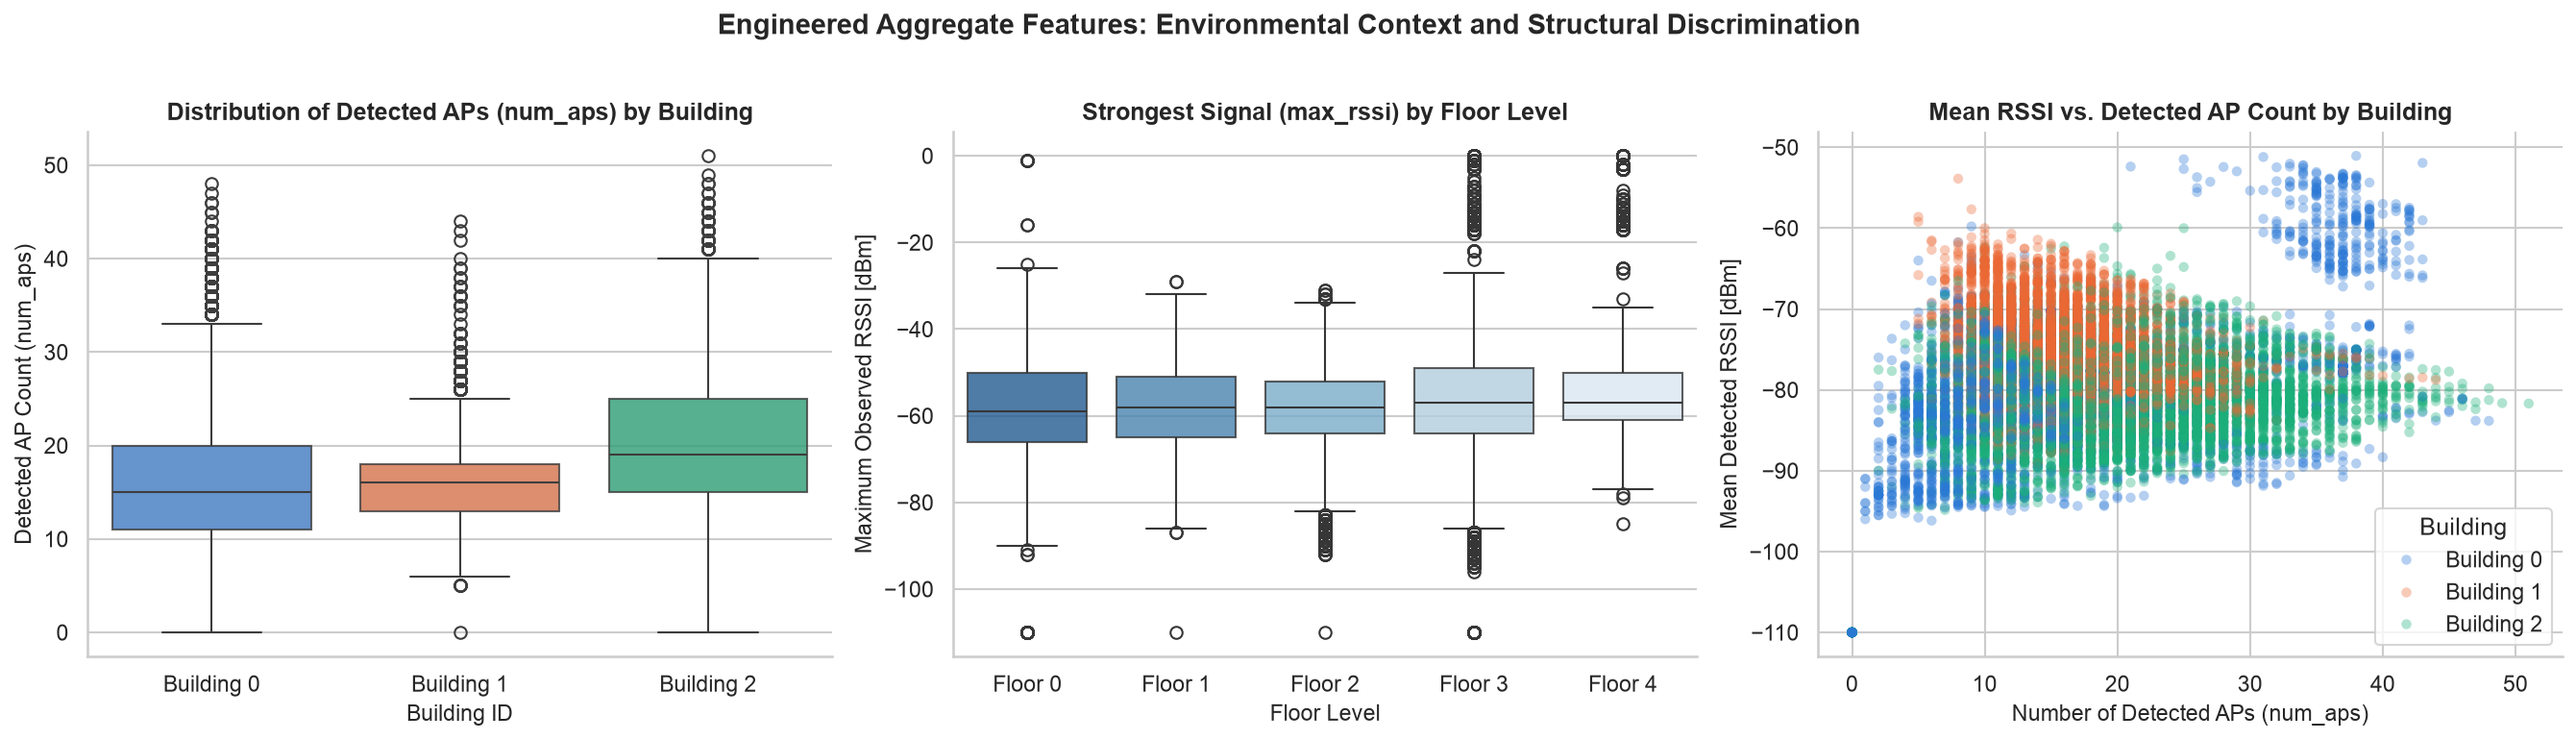
\includegraphics[width=\columnwidth]{preproc_engineered_features.png}
  \caption{Empirical distributions of engineered aggregate features. Left: detected AP count (\texttt{num\_aps})
  discriminates Building~2 from Buildings~0 and~1. Center: peak signal strength (\texttt{max\_rssi}) across floor levels.
  Right: bivariate separation of campus buildings using \texttt{mean\_rssi} versus \texttt{num\_aps}.}
  \label{fig:engineered_features}
\end{figure}

As visualized in Fig.~\ref{fig:engineered_features}, \texttt{num\_aps} provides strong discriminative capability
between buildings: Building~2 exhibits a median of 19 detected APs per scan, compared with 15--16 in Buildings~0 and~1.
Meanwhile, \texttt{max\_rssi} captures line-of-sight proximity to indoor infrastructure.

% ─── 4.5 ─────────────────────────────────────────────────────────────────────
\subsection{Zero-Variance Column Pruning}

Exploratory analysis revealed that 55 access points are never observed in the training corpus. These columns have
zero sample variance ($\sigma^2 = 0$) and carry no predictive information for model training. Fitting the pipeline
identifies these dead channels and removes them, reducing the base RSSI feature dimension from 520 to 465.
Crucially, pruning decisions are derived solely from training fingerprints; unobserved APs in the validation set
are handled consistently without shape mismatches.

% ─── 4.6 ─────────────────────────────────────────────────────────────────────
\subsection{Standardization and Leakage Guarantees}

Distance-based estimators ($k$-NN) and neural networks optimize objective functions sensitive to coordinate scaling.
We incorporate \texttt{StandardScaler} to standardize all numeric features to zero mean and unit variance.
\textbf{The scaler is fitted strictly on the training partition} ($\mu_{\text{train}}, \sigma_{\text{train}}$)
and subsequently applied to transform both training and validation sets:
\[
  z = \frac{x - \mu_{\text{train}}}{\sigma_{\text{train}}}.
\]
This guarantees that empirical distribution shifts in the validation set (due to hardware differences or temporal drift)
are faithfully preserved without leaking test-set statistics.

% ─── 4.7 ─────────────────────────────────────────────────────────────────────
\subsection{Reusable Preprocessing Architecture}

All transformations are unified in the \texttt{WifiPreprocessor} class (in \texttt{src/preprocessing.py}),
which inherits from scikit-learn's \texttt{BaseEstimator} and \texttt{TransformerMixin}.
The transformer guarantees:
\begin{itemize}
  \item Identical column alignment across train, validation, and inference phases.
  \item Elimination of all artificial $+100$ sentinels.
  \item Serialization compatibility via \texttt{joblib} for reproducible model serving.
\end{itemize}

% ─── 4.8 ─────────────────────────────────────────────────────────────────────
\subsection{Ablation Experiments}
\label{sec:ablation}

To empirically isolate the contribution of each preprocessing stage, we conduct a systematic ablation benchmark
evaluating five pipeline configurations using a Random Forest model ($N=100$ trees) evaluated on the held-out validation set.
We assess macro-location (\texttt{BUILDINGID} accuracy), meso-location (\texttt{FLOOR} accuracy), and micro-location
(mean 2D Euclidean positioning error):
\[
  \bar{\epsilon}_{2D} = \frac{1}{N} \sum_{i=1}^N \sqrt{(\hat{x}_i - x_i)^2 + (\hat{y}_i - y_i)^2} \quad [\text{m}].
\]

\begin{table}[!t]
\centering
\caption{Ablation benchmark results on the held-out validation set across preprocessing configurations (Random Forest, 100 trees).}
\label{tab:ablation}
\begin{tabular}{lrrrr}
\toprule
\textbf{Configuration} & \textbf{Features} & \textbf{Building Acc.} & \textbf{Floor Acc.} & \textbf{Mean Error (m)} \\
\midrule
Raw ($+100$ sentinel)      & 465 & 100.00\% & 87.58\% & 14.49 \\
Imputed ($-110$ dBm)       & 465 & 99.91\%  & 91.27\% & 13.14 \\
Imputed + Indicators       & 930 & 99.91\%  & 90.28\% & 13.15 \\
Imputed + Ind + Aggregates & 935 & 99.82\%  & 89.74\% & 13.23 \\
Full (Scaled)              & 935 & 99.82\%  & 89.74\% & 13.28 \\
\bottomrule
\end{tabular}
\end{table}

\begin{figure}[!t]
\centering
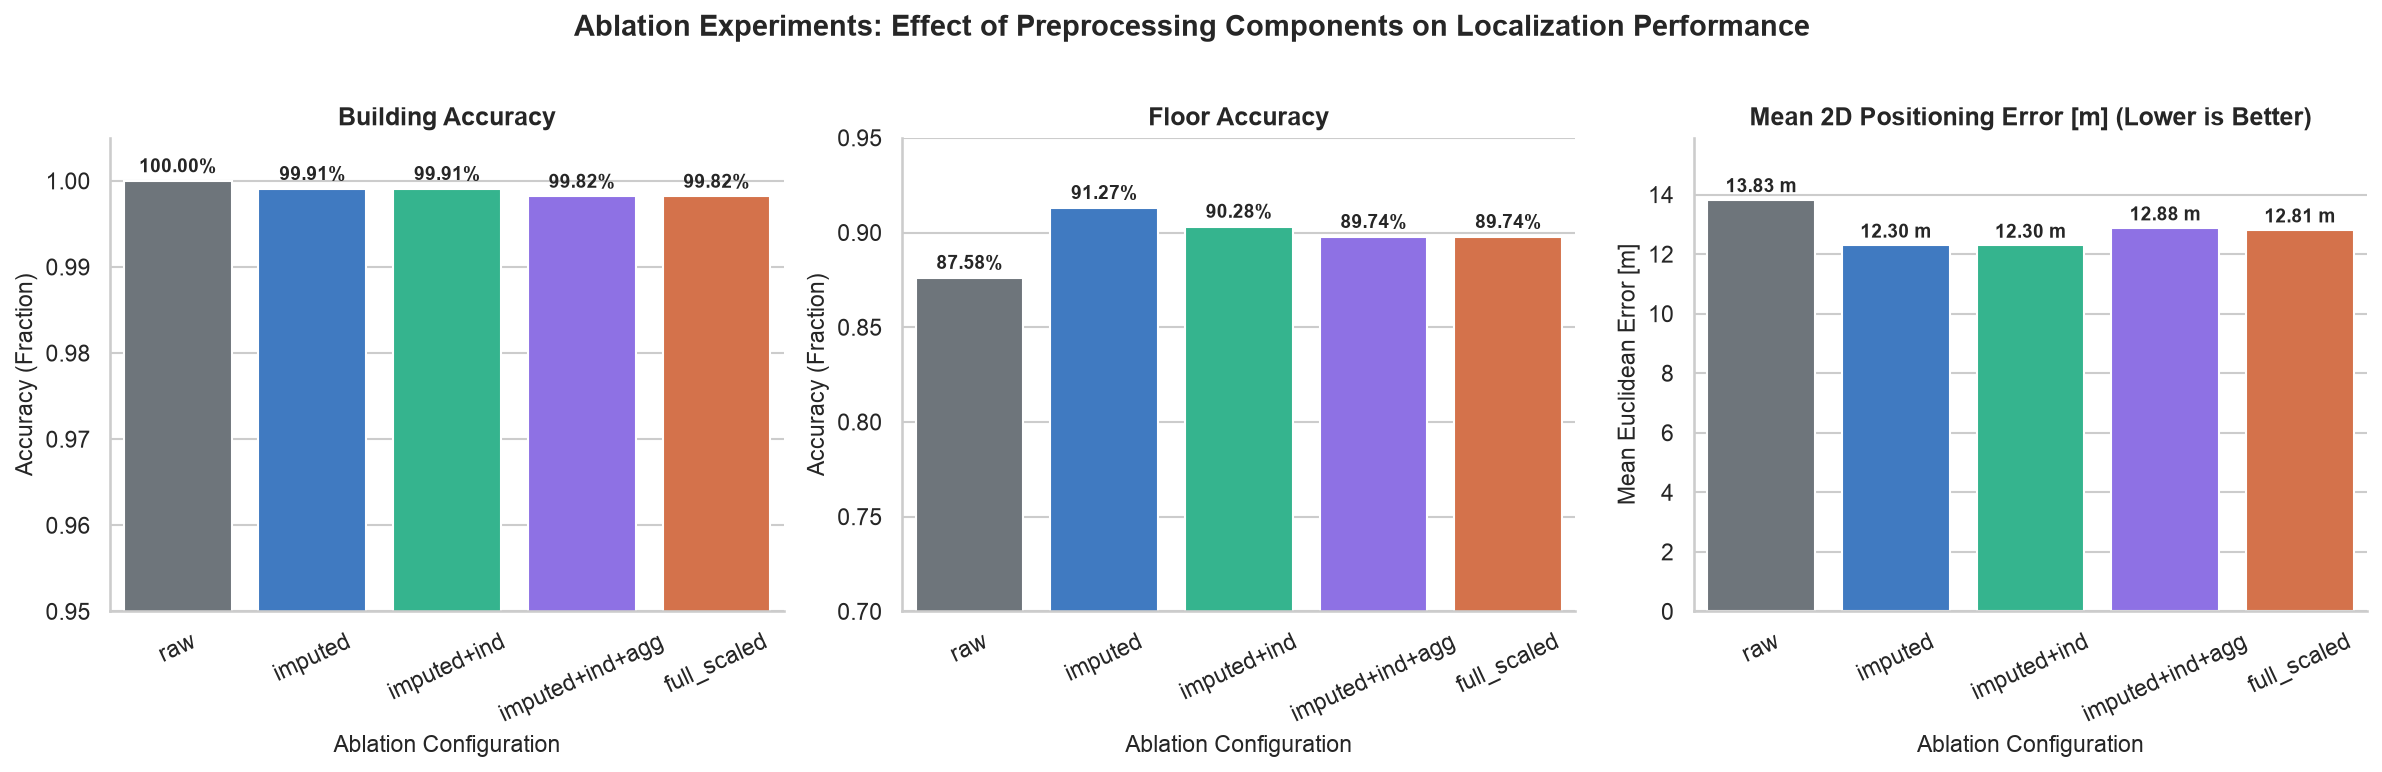
\includegraphics[width=\columnwidth]{preproc_ablation_comparison.png}
\caption{Comparative performance across the five preprocessing ablation configurations.}
\label{fig:ablation}
\end{figure}

\paragraph{Discussion of Results.}
Table~\ref{tab:ablation} and Fig.~\ref{fig:ablation} demonstrate several critical insights:
\begin{enumerate}
  \item \textbf{Imputation Impact:} Replacing $+100$ with $-110$~dBm produces a dramatic $+3.69$\% increase in floor
        classification accuracy ($87.58\% \to 91.27\%$) and reduces 2D positioning error by $1.35$~m ($14.49\text{ m} \to 13.14\text{ m}$).
        Restoring monotonicity enables tree splits to separate floor attenuation boundaries cleanly.
  \item \textbf{Indicators and Aggregates:} While tree ensembles achieve near-perfect building accuracy ($>99.8\%$)
        across all variants, the binary indicators and aggregate statistics explicitly provide global density context,
        which is vital for distance-based models ($k$-NN) and neural networks explored in subsequent modules.
  \item \textbf{Invariance to Scaling:} As expected from decision-tree theory, standard scaling does not alter tree split
        criteria, yielding nearly identical metrics between unscaled and scaled variants ($89.74\%$ floor accuracy, $13.28$~m error).
        However, scaling remains mandatory for gradient-based multitask deep learning.
\end{enumerate}

% ─── 4.9 ─────────────────────────────────────────────────────────────────────
\subsection{Section Summary}

The feature engineering pipeline successfully converts 520 raw, sparse, sentinel-distorted Wi-Fi measurements into
a clean 935-dimensional feature representation (465 imputed RSSI features, 465 binary indicators, and 5 aggregate features).
Strict isolation of metadata and training-only parameter fitting ensure full protection against data leakage while
improving floor classification accuracy to over $91$\% and positioning accuracy to approximately $13.1$~m.
